\documentclass[12pt]{article}
\usepackage{amsmath}
\usepackage{amssymb}
\usepackage{framed}
\usepackage{graphicx}
\voffset=-1.5cm
\oddsidemargin=0.0cm
\textwidth = 470pt
%----------------------------------------------------------------%

% Euclidean Distance
% Squared Euclidean Distance
% City Block Distance
%----------------------------------------------------------------%
\begin{document}
\author{Kevin O'Brien}
\title{Cluster Analysis - Partitioning Around Medoids (k-means)}

\newpage
\section*{PAM: Partitioning Around Medoids}
\begin{itemize}
\item Unlike the hierarchical clustering methods, techniques like k-means cluster analysis (available through the \texttt{kmeans} function) or partitioning around \textbf{\textit{mediods}}  require that we specify the number of clusters that will be formed in advance. 
\item This method is available through the \texttt{pam} function in the \textbf{\textit{cluster}} library.
\item \texttt{pam} offers some additional diagnostic information about a clustering solution, and provides a nice example of an alternative technique to hierarchical clustering. 
%To use \texttt{pam}, you must first load the cluster library. 
\item You can pass \texttt{pam} a data frame or a distance matrix, as well as the number of clusters you wish to form. 
\item Let's look at the three cluster solution produced by \texttt{pam}:
\end{itemize}
\begin{framed}
\begin{verbatim}
#install.packages("cluster")
library(cluster)

cars.pam = pam(cars,3)
\end{verbatim}
\end{framed}
\begin{itemize}
\item Use the \texttt{summary()}, names() , \texttt{class()} and \texttt{str()} commands to analyse the output of the procedure.
\end{itemize}


\begin{framed}
\begin{verbatim}
> names(cars.pam)
 [1] "medoids"    "id.med"     "clustering" "objective" 
 [5] "isolation"  "clusinfo"   "silinfo"    "diss"      
 [9] "call"       "data"
\end{verbatim}
\end{framed}

\subsection*{Results of Procedure}
\begin{itemize}
\item The medoids (centres in other words) of each of the three clusters
\end{itemize}
\begin{framed}
\begin{verbatim}
> cars.pam$medoids
   Country Car  MPG Weight Drive_Ratio Horsepower
30       7  20 18.2  3.830        2.45        135
37       5  26 29.5  2.135        3.05         68
19       5  16 22.0  2.815        3.70         97
   Displacement Cylinders
30          318         8
37           98         4
19          146         6
>
> cars.pam$id.med
[1] 30 37 19
\end{verbatim}
\end{framed}


\begin{itemize}
\item The cluster assignment for each of the 38 cases.
\end{itemize}
\begin{framed}
\begin{verbatim}
> cars.pam$clustering
 1  2  3  4  5  6  7  8  9 10 11 12 13 14 15 16 17 18 19 
 1  2  2  2  2  2  2  2  2  2  3  3  3  3  3  3  3  3  3 
20 21 22 23 24 25 26 27 28 29 30 31 32 33 34 35 36 37 38 
 3  3  3  2  1  3  1  3  1  1  1  1  1  3  3  3  3  2  1
> table(cars.pam$clustering)

 1  2  3 
 9 11 18 

\end{verbatim}
\end{framed}
\begin{itemize}
\item Summary statistics on the dimensionality of each cluster.
\end{itemize}
\begin{framed}
\begin{verbatim}
> cars.pam$clusinfo
     size max_diss  av_diss  diameter separation
[1,]    9 64.44583 33.85620 106.90893   31.24501
[2,]   11 18.10320 13.25804  31.75348   23.44201
[3,]   18 86.00128 34.71620 113.97993   23.44201
\end{verbatim}
\end{framed}
\begin{itemize}
\item Information used to construct the silohouette plot (forthcoming) is contained in \texttt{cars.pam\$silinfo}
\end{itemize}

\subsection*{Comparison of Results}
\begin{itemize}
\item Let's see if this solution agrees with the \texttt{hclust} solution. 
\item Since pam only looks at one cluster solution at a time, we don't need to use the \texttt{cutree} function as we did with hclust
\item The cluster memberships are stored in the \texttt{clustering} component of the \texttt{pam} object (see below).
%like most R objects, you can use the names function to see what else is available. 
%Further information can be found in the help page for pam.object.


\item We can use \texttt{table()} to compare the results of the \texttt{hclust} and \texttt{pam} solutions:
\begin{framed}
\begin{verbatim}
> cars.pam$clustering
 [1] 1 2 2 2 2 2 2 2 2 2 1 3 3 3 1 1 1 3 3 1 3 1 2
[24] 1 3 1 3 1 1 1 1 1 1 3 3 3 2 1 1
>
> table(groups.3,cars.pam$clustering)
groups.3  1  2  3
       1  8  0  0
       2  0 19  1
       3  0  0 10
\end{verbatim}
\end{framed}
\item The solutions seem to agree, except for 1 observations that \texttt{hclust} put in group 2 and \texttt{pam} put in group 3. Which observations was it?
\end{itemize}

\begin{framed}
\begin{verbatim}
> cars$Car[groups.3 != cars.pam$clustering]
[1] Audi 5000
\end{verbatim}
\end{framed}
%Notice how easy it is to get information like this due to the power of R's subscripting operations.
\newpage
\begin{itemize}
\item One novel feature of \texttt{pam} is that it finds observations from the original data that are typical of each cluster in the sense that they are closest to the center of the cluster. 
\item The indexes of the medoids are stored in the \texttt{id.med} component of the \texttt{pam} object, so we can use that component as a subscript into the vector of car names to see which ones were selected:
\end{itemize}
\begin{framed}
\begin{verbatim}
> cars$Car[cars.pam$id.med]
> cars$Car[cars.pam$id.med]
[1] Dodge St Regis    Dodge Omni        Ford Mustang Ghia
\end{verbatim}
\end{framed}
\subsection*{Exercises}
Try out the PAM procedure on the European Jobs Data Set, with a 3 and 4 cluster solution respectively.
\begin{itemize}
\item What are the medoids for the 3 cluster solution?
\item What are the medoids for the 4 cluster solution?
\item For both solutions, how many are in each cluster?
\end{itemize}
\newpage
\subsection*{Silhouette Plot}
\begin{itemize}
\item Another feature available with \texttt{pam} is a plot known as a \textbf{\textit{silhouette plot}}. 
\item First, a measure is calculated for each observation to see how well it fits into the cluster that it's been assigned to. 
This is done by comparing how close the object is to other objects in its own cluster with how close it is to objects in other clusters. 
%(A complete description can be found in the help page for silhouette.) 
\item Values near one mean that the observation is well placed in its cluster; values near 0 mean that it's likely that an observation might really belong in some other cluster. Within each cluster, the value for this measure is displayed from smallest to largest. 
\item If the silhouette plot shows values close to one for each observation, the fit was good; if there are many observations closer to zero, it's an indication that the fit was not good. 
\item The sihouette plot is very useful in locating groups in a cluster analysis that may not be doing a good job; in turn this information can be used to help select the proper number of clusters. 
\item For the current example, here's the silhouette plot for the three cluster \texttt{pam} solution, produced by the command
\end{itemize}
\bigskip
\noindent \textbf{Summary}\\
Silhouette Plot shows for each cluster:

\begin{itemize}
\item the number of plots per cluster = number of horizontal lines, also given in the right hand column,
\item the means similarity of each plot to its own cluster minus the mean similarity to the next most similar cluster (given by the length of the lines) with the mean in the right hand column, and
\item the average silhouette width
\end{itemize}

\newpage
\begin{framed}
\begin{verbatim}
clusplot(cars.pam)
plot(cars.pam) # both plots Sequentially
\end{verbatim}
\end{framed}
\begin{figure}[h!]
\centering
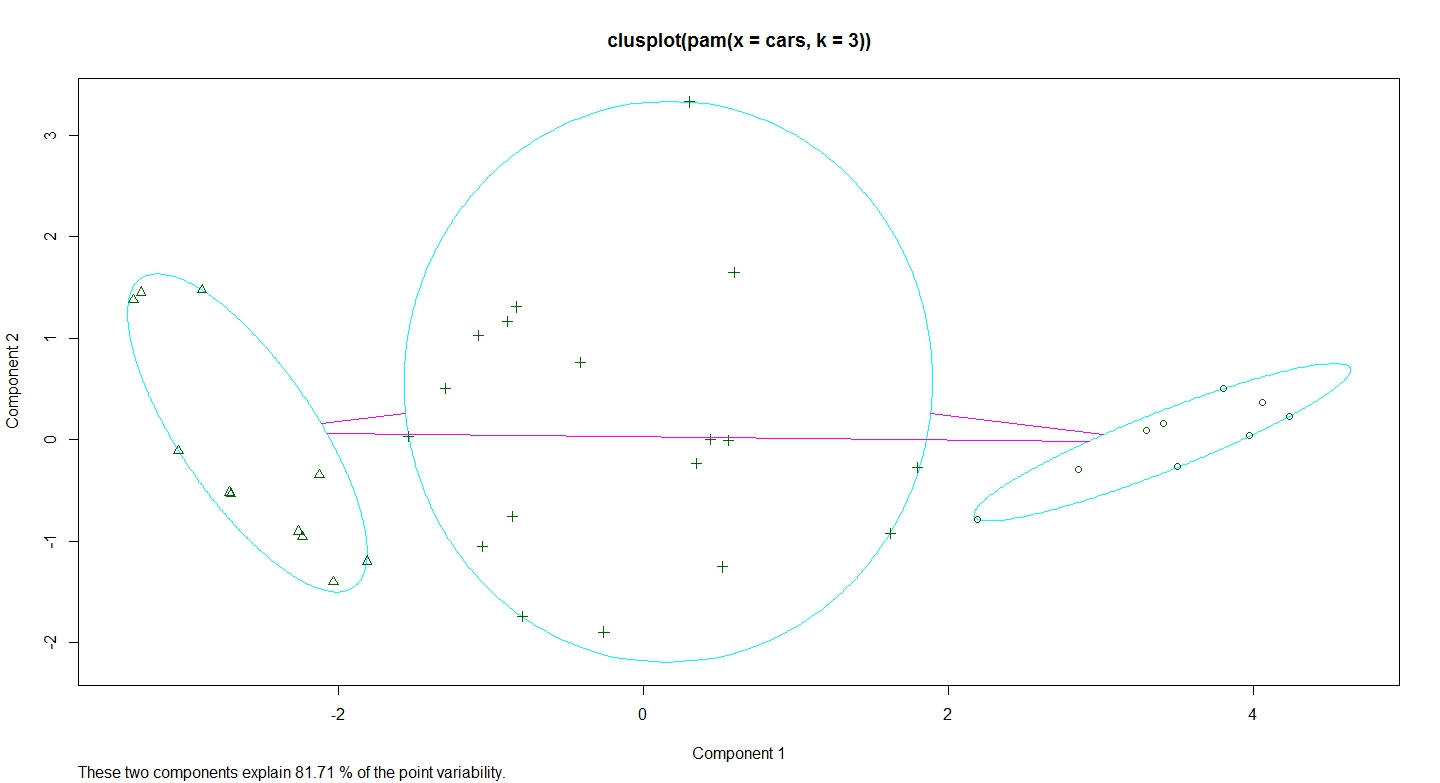
\includegraphics[width=0.8\linewidth]{./ClusPlot}

\label{fig:ClusPlot}
\end{figure}

\begin{figure}[h!]
\centering
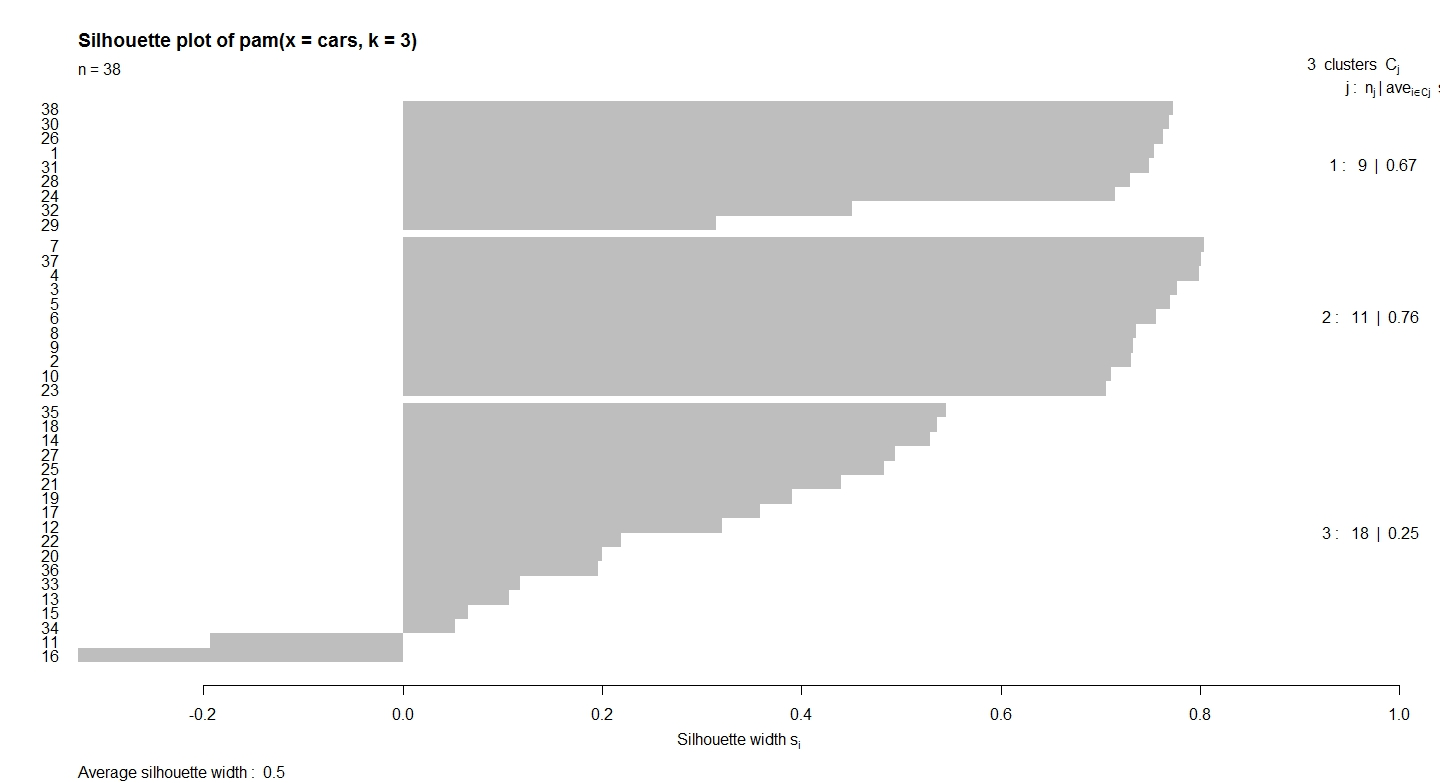
\includegraphics[width=0.9\linewidth]{./SiloPlot}

\label{fig:SiloPlot}
\end{figure}

The plot indicates that there is a good structure to the clusters, with most observations seeming to belong to the cluster that they're in. 

\subsection*{Average Silhouette Width}
There is a summary measure at the bottom of the plot labeled "\textbf{\textit{Average Silhouette Width}}". This table shows how to use the value:
\bigskip

\begin{tabular}{|c|l|}
\hline
Range 	& Interpretation \\ \hline \hline
0.71-1.0 &	A strong structure has been found \\ \hline
0.51-0.70&  	A reasonable structure has been found \\ \hline
0.26-0.50&	The structure is weak and could be artificial \\ \hline
$<$ 0.25&	No substantial structure has been found \\ \hline
\end{tabular} 
\subsection*{Exercises}
Try out the PAM procedure on the \textbf{\textit{cars}} Data Set, with a 4 and 5 cluster solution respectively.
\begin{itemize}
\item What is the average silouette width for the 4 cluster solution?
\item What is the average silouette width for the 5 cluster solution?
\end{itemize}
Try out the PAM procedure on the \textbf{\textit{European Jobs}} Data Set, with a 4 and 5 cluster solution respectively.
\begin{itemize}
\item What is the average silouette width for the 4 cluster solution?
\item What is the average silouette width for the 5 cluster solution?
\end{itemize}
\newpage
\subsection*{Creating Silhouette Plots for Other Solutions}
\begin{itemize}
\item To create a silhouette plot for a particular solution derived from a hierarchical cluster analysis, the \texttt{silhouette} function can be used. 
\item This function takes the appropriate output from cutree along with the distance matrix used for the clustering. 
\item So to produce a silhouette plot for our 4 group hierarchical cluster (not shown), we could use the following statements:
\end{itemize}
\begin{framed}
\begin{verbatim}
plot(silhouette(cutree(cars.hclust,4),cars))
\end{verbatim}
\end{framed}

\end{document}